% Included by chapters/intro.tex.
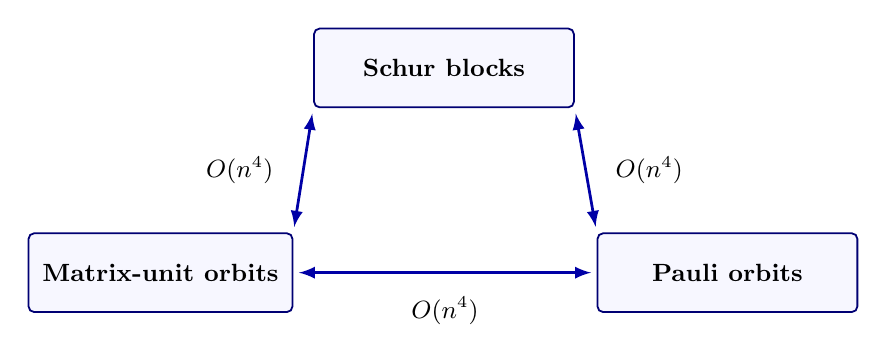
\begin{tikzpicture}[
    font=\small,
    representation/.style={
        draw=blue!45!black,
        fill=blue!3,
        rounded corners=2pt,
        line width=0.65pt,
        minimum width=3.3cm,
        minimum height=1.0cm,
        align=center,
        inner sep=5pt
    },
    conversion/.style={
        <->,
        >=latex,
        draw=blue!65!black,
        line width=1pt,
        shorten <=2pt,
        shorten >=2pt
    }
]
    \node[representation] (schur) at (0,2.6)
        {\textbf{Schur blocks}};
    \node[representation] (matrix) at (-3.6,0)
        {\textbf{Matrix-unit orbits}};
    \node[representation] (pauli) at (3.6,0)
        {\textbf{Pauli orbits}};

    \draw[conversion] (schur.south west) --
        node[midway, left=7pt] {$O(n^4)$}
        (matrix.north east);
    \draw[conversion] (schur.south east) --
        node[midway, right=7pt] {$O(n^4)$}
        (pauli.north west);
    \draw[conversion] (matrix.east) --
        node[midway, below=5pt] {$O(n^4)$}
        (pauli.west);
\end{tikzpicture}
